% !TEX program = pdflatex
% Overleaf: set the project compiler to pdfLaTeX (Menu -> Compiler -> pdfLaTeX).
\documentclass[11pt]{article}

\usepackage[T1]{fontenc}
\usepackage[utf8]{inputenc}
\usepackage{lmodern}
\usepackage[margin=1in]{geometry}
\usepackage{amsmath,amssymb}
\usepackage{booktabs}
\usepackage{array}
\usepackage{graphicx}
\usepackage{float}
\usepackage{tikz}
\usepackage{parskip}
\usepackage{xcolor}
\usepackage[hidelinks]{hyperref}

\newcommand{\todo}[1]{\textcolor{gray}{\textit{#1}}}

\title{%
  ESE~5700: Digital Integrated Circuits and VLSI Fundamentals\\
  \large Project~1, Part~1: The 6T Bitcell%
}
\author{Tyrone Marhguy \and Victor Wanjohi}
\date{University of Pennsylvania \\ Due: 9/29/2026}

\begin{document}
\maketitle

\begin{center}
  
\includegraphics[width=0.45\linewidth]{media/penn-logo.png}
\end{center}

\section*{Team and contributions}
\begin{tabular}{@{}ll@{}}
\toprule
\textbf{Member} & \textbf{Contributions (this part)} \\
\midrule
Tyrone Marhguy & \todo{TBD} \\
Victor Wanjohi & \todo{TBD} \\
\bottomrule
\end{tabular}

\noindent Both team members are responsible for understanding the full design and report.

\newpage

\section*{1.~Sizing ($\beta$ and $\gamma$)}
\subsection*{Hand analysis}
\begin{figure}[H]
  \centering
  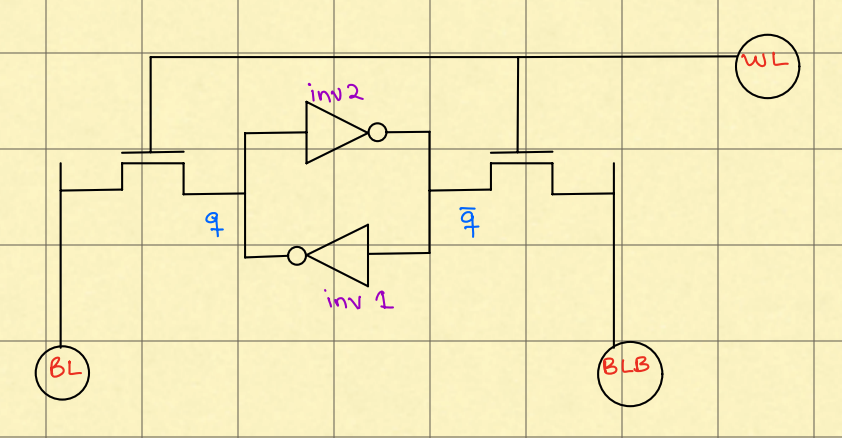
\includegraphics[width=0.7\linewidth]{media/part1/6t-cell-wl-bl-inv12-q-qb.png}
  \caption{6T cell read-disturb setup: $Q=0$ stored, wordline asserted,
  bitlines precharged (hand sketch).}
\end{figure}

\subsubsection*{Read stability}
Assume the stored state $Q=0$ ($\overline{Q}\approx V_{DD}$) for
read-stability analysis. With $Q=0$ the ``0'' node is pulled down by
the NMOS inside INV1 while the bitline (precharged to $V_{DD}$) drives
current through the pass-gate, so the disturbed node follows an
approximate voltage-divider model:
\begin{equation}
\frac{V_Q}{V_{DD}} = \frac{R_{\mathrm{PD1}}}{R_{\mathrm{PG}}+R_{\mathrm{PD1}}}
= \frac{1}{1+R_{\mathrm{PG}}/R_{\mathrm{PD1}}}.
\end{equation}
From transistor physics $R_T\propto 1/W_T$ at fixed $L$. Defining the
cell ratio $\beta=(W/L)_{\mathrm{PD}}/(W/L)_{\mathrm{PG}}
=W_{\mathrm{PD}}/W_{\mathrm{PG}}$ gives
$\beta\approx R_{\mathrm{PG}}/R_{\mathrm{PD}}$, hence
\begin{equation}
\frac{V_Q}{V_{DD}} \approx \frac{1}{1+\beta},
\qquad V_Q \approx \frac{V_{DD}}{1+\beta}:
\end{equation}
a larger $\beta$ lowers the read-disturb bump. Whether that bump flips
the cell is set by the inverter switching voltage $V_M$
($V_{\mathrm{in}}=V_{\mathrm{out}}$), where both devices conduct.
\begin{figure}[H]
  \centering
  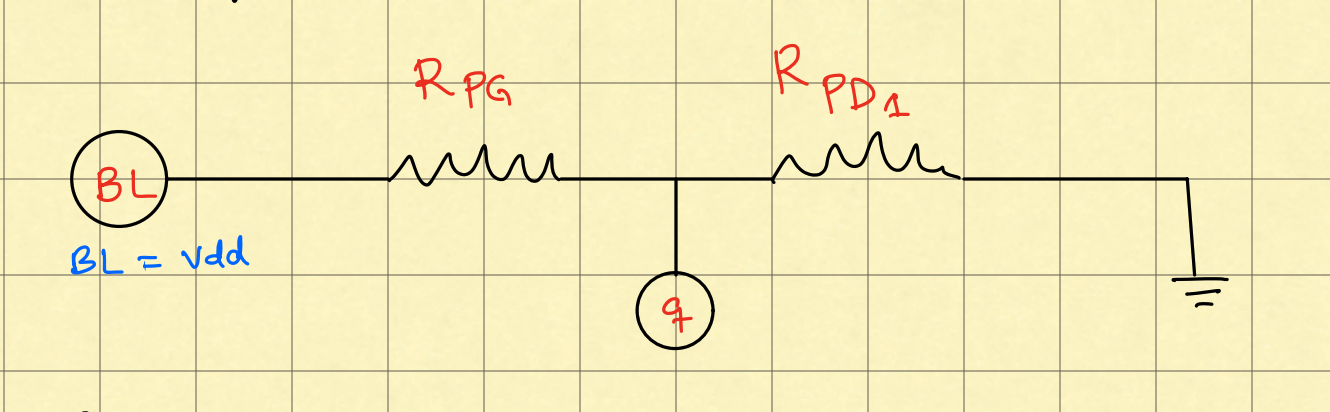
\includegraphics[width=0.7\linewidth]{media/part1/voltage_div_diagram.png}
  \caption{Approximate resistive divider for the read disturb:
  precharged bitline through $R_{\mathrm{PG}}$ against the pull-down
  $R_{\mathrm{PD1}}$ to ground (hand sketch).}
\end{figure}

Current balance at the equilibrium disturb voltage: neglecting gate
leakage, KCL gives $I_{\mathrm{PD}}=I_{\mathrm{PG}}$. The pass-gate has
$D=G=V_{DD}$, $S=V_Q$, so $V_{DS}=V_{GS}=V_{DD}-V_Q$ and
$V_{DS}>V_{GS}-V_{Tn}$ always: saturation, with
$I_{\mathrm{PG}}=\tfrac{1}{2}k_{\mathrm{PG}}(V_{GS}-V_{Tn})^2$ and
$k_{\mathrm{PG}}=\mu_n C_{ox}(W/L)_{\mathrm{PG}}$.
The pull-down (pd1) has $V_D=V_Q$, $V_G\approx V_{DD}$, $V_S=0$, so
$V_{DS}=V_Q<V_{GS}-V_{Tn}$: triode, with
$I_{\mathrm{PD}}=k_{\mathrm{PD}}[(V_{GS}-V_{Tn})V_{DS}-V_{DS}^2/2]$.
Equating the two with $E=V_{DD}-V_{Tn}$ yields
\begin{equation}
V_Q^2(1+\beta)+V_Q(-2E-2E\beta)+E^2=0
\quad\Rightarrow\quad
V_Q = E\left(1\pm\sqrt{\frac{\beta}{1+\beta}}\right),
\end{equation}
of which the positive root exceeds $V_{DD}-V_{Tn}$ and is inconsistent
with the assumed saturated pass-gate / triode pull-down, leaving
\begin{equation}
V_Q = (V_{DD}-V_{Tn})\left(1-\sqrt{\frac{\beta}{1+\beta}}\right).
\end{equation}
This assumes ideal long-channel square-law behavior, equal NMOS
thresholds, and negligible body effect.

The disturbed node $Q$ drives INV2, whose switching point satisfies
$I_{DN}=|I_{DP}|$ with both devices in saturation:
\begin{equation}
V_M = \frac{V_{Tn}+B\,(V_{DD}-|V_{Tp}|)}{1+B},
\qquad B=\sqrt{\frac{k_P}{k_N}}
      =\sqrt{\frac{\gamma\,\mu_p}{\beta\,\mu_n}},
\label{eq:vm}
\end{equation}
with $k_P/k_N=\mu_p C_{ox}(W/L)_{\mathrm{PU}}/
\big(\mu_n C_{ox}(W/L)_{\mathrm{PG}}\big)$,
$\beta=(W/L)_{\mathrm{PD}}$, and $\gamma=(W/L)_{\mathrm{PG}}$ as written
in the hand-note derivation, so $V_M$ depends on the supply, the
threshold voltages, and the
relative PMOS/NMOS strengths. Read stability requires $V_Q<V_M$:
\begin{equation}
(V_{DD}-V_{Tn})\left(1-\sqrt{\frac{\beta}{1+\beta}}\right)
<
\frac{V_{Tn}+\sqrt{\frac{\mu_p\gamma}{\mu_n\beta}}\,(V_{DD}-|V_{Tp}|)}
     {1+\sqrt{\frac{\mu_p\gamma}{\mu_n\beta}}}.
\end{equation}
Increasing $\beta$ strengthens the pull-down relative to the pass-gate
and lowers the disturb voltage, but $\beta$ also moves $V_M$ and costs
area: the final cell ratio is not selected by minimizing $V_Q$ alone.
\subsubsection*{Write stability}
Assume the stored state $Q = 1$ ($\overline{Q} \approx 0$) for the write
analysis, with a 0 written through BL. With BL driven to $0\,\mathrm{V}$ and
WL at $V_{DD}$, the pass-gate pulls the ``1'' node down while the PMOS inside
INV1, still on because $\overline{Q} \approx 0$, pulls it up to $V_{DD}$. The
written node therefore follows an approximate voltage-divider model:
\begin{equation}
  \frac{V_Q}{V_{DD}}
  = \frac{R_{\mathrm{PG}}}{R_{\mathrm{PG}} + R_{\mathrm{PU1}}}
  = \frac{1}{1 + R_{\mathrm{PU1}}/R_{\mathrm{PG}}}.
  \label{eq:w-divider}
\end{equation}
From transistor physics $R_T \propto 1/(\mu_T W_T)$ at fixed $L$. The two
devices are of opposite type, so the mobility ratio does not cancel as it does
in the read divider. Defining the pull-up ratio
$\gamma = (W/L)_{\mathrm{PU}}/(W/L)_{\mathrm{PG}}
        = W_{\mathrm{PU}}/W_{\mathrm{PG}}$
gives $R_{\mathrm{PU1}}/R_{\mathrm{PG}} \approx \mu_n/(\mu_p\gamma)$, hence
\begin{equation}
  \frac{V_Q}{V_{DD}} \approx \frac{1}{1 + \dfrac{\mu_n}{\mu_p\gamma}},
  \qquad
  V_Q \approx V_{DD}\,\frac{\mu_p\gamma}{\mu_n + \mu_p\gamma}:
  \label{eq:w-divider-gamma}
\end{equation}
a smaller $\gamma$ lowers the written node. Whether it falls far enough to
flip the cell is set by the switching voltage $V_M$
($V_{\mathrm{in}} = V_{\mathrm{out}}$) of INV2, which $Q$ drives.
 
\begin{figure}[h]
  \centering
  % Replace this drawing with \includegraphics of a hand sketch if the
  % assignment asks for one.
  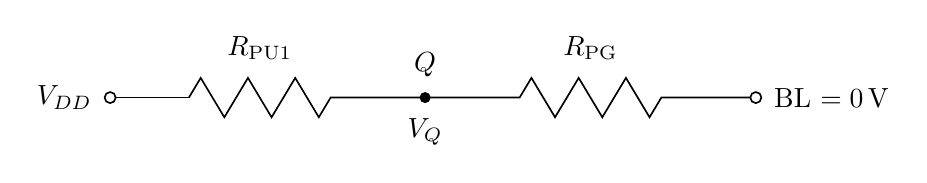
\begin{tikzpicture}[line width=0.6pt, x=1cm, y=1cm]
    % supply terminal
    \draw (0,0) circle (2pt);
    \node[left=3pt] at (0,0) {$V_{DD}$};
    \draw (0.07,0) -- (1,0);
    % R_PU1
    \draw (1,0) -- ++(0.15,0.25) -- ++(0.3,-0.5) -- ++(0.3,0.5)
          -- ++(0.3,-0.5) -- ++(0.3,0.5) -- ++(0.3,-0.5)
          -- ++(0.15,0.25) -- (4,0);
    \node[above] at (1.9,0.35) {$R_{\mathrm{PU1}}$};
    % node Q
    \fill (4,0) circle (2pt);
    \node[above=4pt] at (4,0) {$Q$};
    \node[below=4pt] at (4,0) {$V_Q$};
    % R_PG
    \draw (4,0) -- (5.2,0) -- ++(0.15,0.25) -- ++(0.3,-0.5) -- ++(0.3,0.5)
          -- ++(0.3,-0.5) -- ++(0.3,0.5) -- ++(0.3,-0.5)
          -- ++(0.15,0.25) -- (8.13,0);
    \node[above] at (6.1,0.35) {$R_{\mathrm{PG}}$};
    % bitline terminal
    \draw (8.2,0) circle (2pt);
    \node[right=3pt] at (8.2,0) {BL $= 0\,\mathrm{V}$};
  \end{tikzpicture}
  \caption{Approximate resistive divider for the write: supply through
    $R_{\mathrm{PU1}}$ against the pass-gate $R_{\mathrm{PG}}$ to the
    $0\,\mathrm{V}$ bitline.}
  \label{fig:w-divider}
\end{figure}
 
Current balance at the equilibrium write voltage: neglecting gate leakage,
KCL gives $I_{\mathrm{PU}} = I_{\mathrm{PG}}$. The pass-gate has
$G = V_{DD}$, $S = \mathrm{BL} = 0$ and $D = Q$, so $V_{GS} = V_{DD}$ and
$V_{DS} = V_Q < V_{GS} - V_{Tn}$ at the equilibrium point: triode, with
$I_{\mathrm{PG}} = k_{\mathrm{PG}}\bigl[(V_{DD} - V_{Tn})V_Q - V_Q^2/2\bigr]$
and $k_{\mathrm{PG}} = \mu_n C_{ox}(W/L)_{\mathrm{PG}}$. The pull-up (pu1) has
$S = V_{DD}$, $G = \overline{Q} \approx 0$ and $D = Q$, so $V_{SG} = V_{DD}$
and $V_{SD} = V_{DD} - V_Q > V_{SG} - |V_{Tp}|$ as long as $V_Q < |V_{Tp}|$:
saturation, with
$I_{\mathrm{PU}} = \tfrac{1}{2}k_{\mathrm{PU}}(V_{DD} - |V_{Tp}|)^2$ and
$k_{\mathrm{PU}} = \mu_p C_{ox}(W/L)_{\mathrm{PU}}$. Equating the two with
$E = V_{DD} - V_{Tn}$, $F = V_{DD} - |V_{Tp}|$ and
$k_{\mathrm{PU}}/k_{\mathrm{PG}} = \gamma\,\mu_p/\mu_n$ yields
\begin{equation}
  V_Q^{2} - 2E\,V_Q + \gamma\frac{\mu_p}{\mu_n}F^{2} = 0
  \quad\Rightarrow\quad
  V_Q = E \pm \sqrt{E^{2} - \gamma\frac{\mu_p}{\mu_n}F^{2}},
  \label{eq:w-quadratic}
\end{equation}
of which the positive root exceeds $V_{DD} - V_{Tn}$ and is inconsistent with
the assumed triode pass-gate, leaving
\begin{equation}
  V_Q = (V_{DD} - V_{Tn})
        - \sqrt{(V_{DD} - V_{Tn})^{2}
                - \gamma\frac{\mu_p}{\mu_n}\bigl(V_{DD} - |V_{Tp}|\bigr)^{2}}.
  \label{eq:w-vq}
\end{equation}
This assumes ideal long-channel square-law behavior, a saturated pull-up
($V_Q < |V_{Tp}|$), an ideal $0\,\mathrm{V}$ bitline, and no help from PG2
pulling $\overline{Q}$ up.
 
The written node $Q$ drives INV2, whose switching point $V_M$ is the one in
Eq.~\eqref{eq:vm}, with $B = \sqrt{\gamma\mu_p/(\beta\mu_n)}$. Write stability requires
$V_Q < V_M$:
\begin{equation}
  (V_{DD} - V_{Tn})
  - \sqrt{(V_{DD} - V_{Tn})^{2}
          - \gamma\frac{\mu_p}{\mu_n}\bigl(V_{DD} - |V_{Tp}|\bigr)^{2}}
  \;<\;
  \frac{V_{Tn} + \sqrt{\dfrac{\mu_p\gamma}{\mu_n\beta}}
        \bigl(V_{DD} - |V_{Tp}|\bigr)}
       {1 + \sqrt{\dfrac{\mu_p\gamma}{\mu_n\beta}}}.
  \label{eq:w-condition}
\end{equation}
Equation~\eqref{eq:w-vq} holds only while the pull-up is saturated,
$V_Q < |V_{Tp}|$. With the values used here $V_M$ is about
$0.37\,\mathrm{V}$, above $|V_{Tp}| = 0.3\,\mathrm{V}$, so
\eqref{eq:w-condition} cannot be solved for $\gamma$ with \eqref{eq:w-vq}
alone. Requiring the stricter $V_Q < V_{Tn}$ keeps \eqref{eq:w-vq} valid when
$V_{Tn} \le |V_{Tp}|$, guarantees that the NMOS of INV2 is off, and gives the
required pull-up ratio in closed form:
\begin{equation}
  \gamma < \frac{\mu_n}{\mu_p}\cdot
  \frac{V_{Tn}\bigl(2V_{DD} - 3V_{Tn}\bigr)}
       {\bigl(V_{DD} - |V_{Tp}|\bigr)^{2}}.
  \label{eq:w-gamma}
\end{equation}
 
At $V_{DD} = 0.8\,\mathrm{V}$, with the placeholder values
$V_{Tn} = |V_{Tp}| = 0.3\,\mathrm{V}$ and $\mu_n/\mu_p = 2$,
\eqref{eq:w-gamma} gives $\gamma < 1.68$. Evaluating \eqref{eq:w-condition}
numerically at $\beta = 2$, with the triode pull-up current beyond
$V_Q = |V_{Tp}|$, relaxes the limit to about $\gamma < 1.9$. For $\gamma = 1$
the divider \eqref{eq:w-divider-gamma} puts $V_Q$ at $0.27\,\mathrm{V}$ and
the current balance \eqref{eq:w-vq} at $0.15\,\mathrm{V}$; the divider is
pessimistic because a saturated pull-up supplies less current than a resistor
would.
 
\begin{table}[h]
  \centering
  \caption{Written-node voltage against pull-up ratio at
    $V_{DD} = 0.8\,\mathrm{V}$, $\mu_n/\mu_p = 2$.}
  \label{tab:w-gamma}
  \begin{tabular}{cccc}
    \hline
    $\gamma$ & $V_Q$ from \eqref{eq:w-vq} (V) & Margin to $V_{Tn}$ (V)
             & Margin to $V_M$ at $\beta = 2$ (V) \\
    \hline
    0.5 & 0.067 & 0.233 & 0.285 \\
    1   & 0.146 & 0.154 & 0.220 \\
    1.5 & 0.250 & 0.050 & 0.126 \\
    2   & 0.40, pull-up in triode & fails & fails \\
    \hline
  \end{tabular}
\end{table}
 
The bound scales directly with the NMOS-to-PMOS strength ratio. FinFET kits
often have a PMOS much closer to the NMOS than the planar assumption of 2,
and that decides whether a one-fin pass-gate can overpower a one-fin pull-up:
 
\begin{table}[h]
  \centering
  \caption{Sensitivity of the write bound to the NMOS-to-PMOS strength ratio.}
  \label{tab:w-strength}
  \begin{tabular}{cccc}
    \hline
    Strength ratio $\mu_n/\mu_p$ & $\gamma$ limit from \eqref{eq:w-gamma}
      & $V_Q$ at $\gamma = 1$ (V) & $V_Q$ at $\gamma = 0.5$ (V) \\
    \hline
    2    & 1.68 & 0.146 & 0.067 \\
    1.5  & 1.26 & 0.211 & 0.092 \\
    1.25 & 1.05 & 0.276 & 0.113 \\
    1    & 0.84 & fails & 0.146 \\
    \hline
  \end{tabular}
\end{table}
 
Reducing $\gamma$ weakens the pull-up relative to the pass-gate and lowers the
written node, but $\gamma$ moves in whole-fin steps, a stronger pass-gate
lowers $\beta$ and loads the bitline, and $\gamma$ also moves $V_M$: the final
pull-up ratio is not selected by minimizing $V_Q$ alone.

\subsection*{Chosen sizes}
\begin{tabular}{@{}lll@{}}
\toprule
\textbf{Device} & $\boldsymbol{(W/L)}$ & \textbf{Notes} \\
\midrule
Pull-down (PD) & \todo{TBD} & \\
Pull-up (PU) & \todo{TBD} & \\
Pass-gate (PG) & \todo{TBD} & \\
$\beta$ & \todo{TBD} & \\
$\gamma$ & \todo{TBD} & \\
\bottomrule
\end{tabular}

\subsection*{$\beta$ sweep (schematic)}
\begin{tabular}{@{}lll@{}}
\toprule
$\boldsymbol{\beta}$ & \textbf{SNM$_{\mathrm{read}}$} & \textbf{Notes} \\
\midrule
\todo{1$\times$} & \todo{TBD} & \\
\todo{1.5$\times$} & \todo{TBD} & \\
\todo{2$\times$} & \todo{TBD} & \\
\bottomrule
\end{tabular}

\noindent Design point selected: \todo{TBD}. Cell kept symmetric.

\begin{figure}[H]
  \centering
  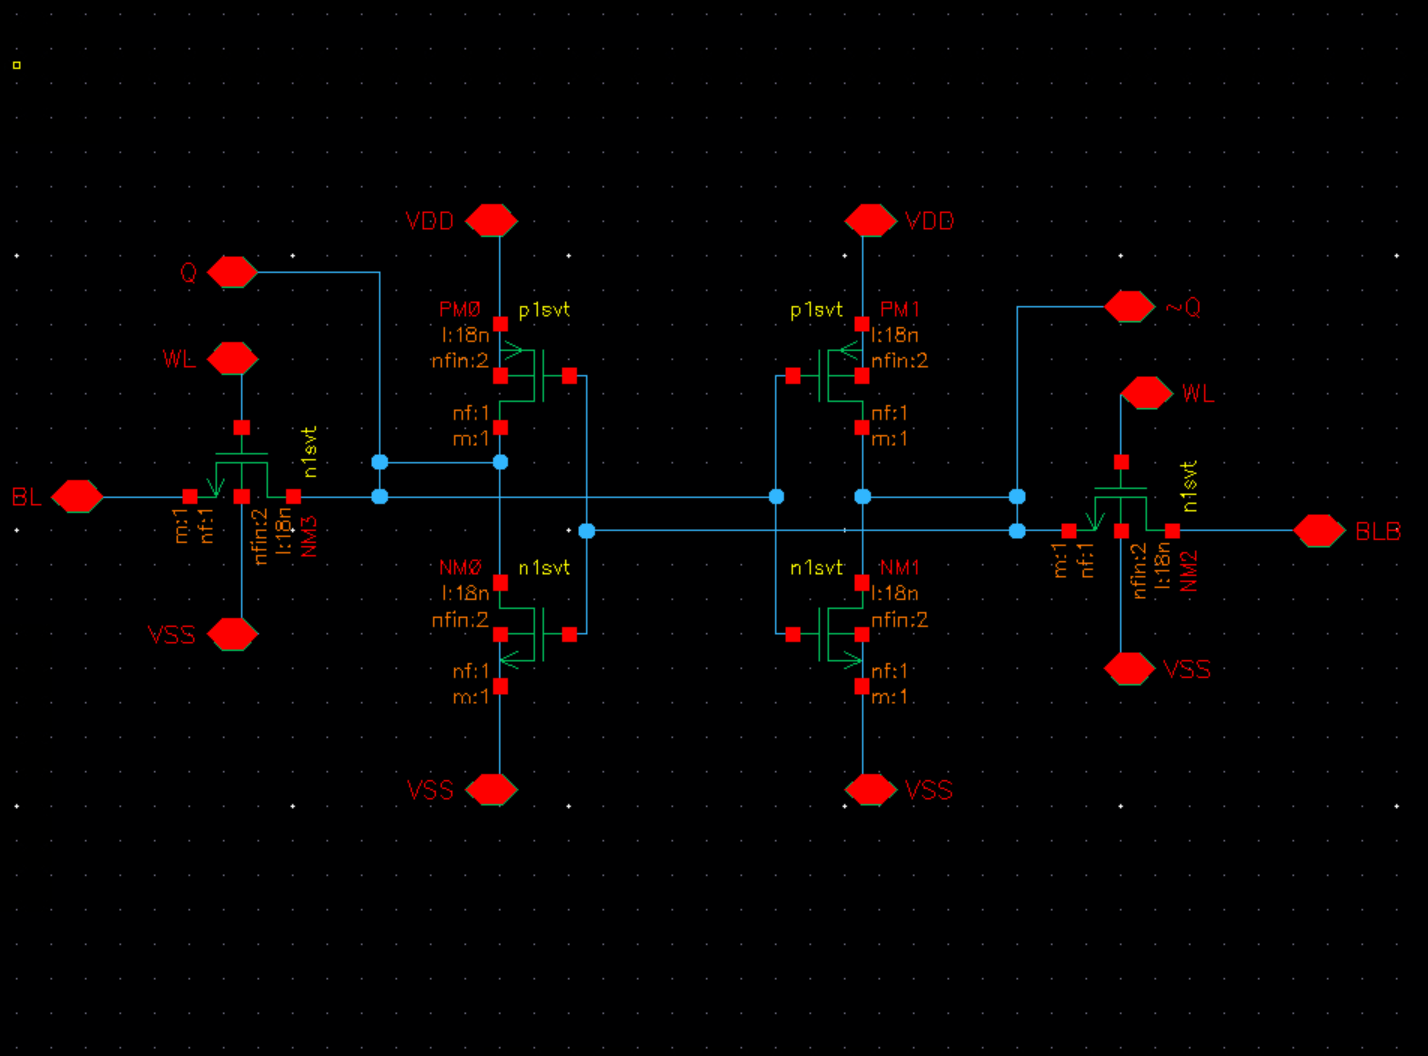
\includegraphics[width=0.7\linewidth]{media/part1/bitcell-schematic.png}
  \caption{6T bitcell schematic with transistor sizes
  (\texttt{proj1\_lib} 6t-sram, Virtuoso capture).}
\end{figure}

\section*{2.~Layout}
\todo{DRC- and LVS-clean layout: wordline horizontal, bitline pair vertical,
tileable for Part~2. Report area in $\mu\mathrm{m}^2$ and $F^2$ ($F = 45\,\mathrm{nm}$).}

\begin{tabular}{@{}ll@{}}
\toprule
\textbf{Metric} & \textbf{Value} \\
\midrule
Cell area & \todo{TBD}~$\mu\mathrm{m}^2$ \\
Cell area in $F^2$ & \todo{TBD}~$F^2$ \\
DRC & \todo{clean / summary} \\
LVS & \todo{clean / summary} \\
\bottomrule
\end{tabular}

% \begin{figure}[H]
%   \centering
%   \includegraphics[width=0.7\linewidth]{media/part1/bitcell-layout.png}
%   \caption{6T bitcell layout.}
% \end{figure}

\section*{3.~Extraction}
\todo{Post-layout parasitic extraction. Report per-cell bitline-node and
wordline-node capacitances (loads for Part~2).}

\begin{tabular}{@{}ll@{}}
\toprule
\textbf{Capacitance} & \textbf{Value} \\
\midrule
$C_{\mathrm{BL}}$ (per cell) & \todo{TBD} \\
$C_{\mathrm{WL}}$ (per cell) & \todo{TBD} \\
\bottomrule
\end{tabular}

\section*{4.~Stability characterization (post-layout, $V_{DD}=1.2\,\mathrm{V}$)}
\subsection*{4a.~Hold SNM}
\todo{Butterfly plot with WL $= 0$; report SNM$_{\mathrm{hold}} = \min(\mathrm{SNM}_L,\mathrm{SNM}_R)$.}

\subsection*{4b.~Read SNM}
\todo{Butterfly plot with WL $= V_{DD}$, BL$=$BLB$=V_{DD}$; report SNM$_{\mathrm{read}}$
and DC voltage of the ``0'' node vs.\ the Section~1 estimate.}

\subsection*{4c.~Write margin}
\todo{Store $Q=1$, WL $= V_{DD}$, BL $= V_{DD}$; sweep BLB; report
$\mathrm{WM}_{\mathrm{BL}} = V_{\mathrm{trip}}$.}

\subsection*{4d.~Cell current}
\todo{Report $I_{\mathrm{cell}}$ from the ``0''-side bitline
(WL $= V_{DD}$, bitlines at $V_{DD}$).}

\subsection*{4e.~Supply dependence}
\begin{tabular}{@{}lll@{}}
\toprule
$\boldsymbol{V_{DD}}$ & \textbf{SNM$_{\mathrm{read}}$} & $\boldsymbol{\mathrm{WM}_{\mathrm{BL}}}$ \\
\midrule
$1.2\,\mathrm{V}$ & \todo{TBD} & \todo{TBD} \\
$0.9\,\mathrm{V}$ & \todo{TBD} & \todo{TBD} \\
$0.6\,\mathrm{V}$ & \todo{TBD} & \todo{TBD} \\
\bottomrule
\end{tabular}

\noindent Still reads and writes at $0.6\,\mathrm{V}$? \todo{yes/no + notes}.

% Waveform / butterfly figures go under media/part1/, e.g.:
% media/part1/butterfly-hold.png
% media/part1/butterfly-read.png
% media/part1/write-margin.png

\section*{5.~Functional check}
\todo{Transient test with ideal WL and precharge pulses; bitline pair loaded by
15 additional per-cell bitline loads. Write 0, read; write 1, read. Show WL, BL,
BLB, $Q$, $\overline{Q}$.}

% \begin{figure}[H]
%   \centering
%   \includegraphics[width=0.95\linewidth]{media/part1/functional-check.png}
%   \caption{Functional write/read waveforms.}
% \end{figure}

\section*{6.~Discussion}
\todo{Short paragraph: what limits the cell, and what you would change for Part~2.}

\section*{Technology note}
All work is done in the Cadence GPDK 18 nm technology (schematic, layout, Spectre/ADE,
DRC/LVS/PEX) at nominal $V_{DD}=1.2\,\mathrm{V}$ unless noted. Characterization above
is post-layout unless a subsection states otherwise.

\end{document}
